\chapter{Návrh}
TODO

\label{kap:navrh} % id kapitoly pre prikaz ref

\section{Požiadavky}

\subsection{Zámer rozšírenia aplikácie!}
Hlavným cieľom tejto práce je zlepšiť použiteľnosť existujúcej aplikácie Prieskumník štruktúr používanej na predmete Logika pre informatikov. Ako bolo už bližšie spomenuté v podkapitole venovanej práve tomuto nástroju \ref{sec:explorer}, súčasná verzia poskytuje iba veľmi obmedzený spôsob vizualizácie a manipulácie s interpretáciami predikátových a funkčných symbolov.

Primárnym zlepšením v tejto oblasti má byť rozšírenie nástroja o grafové editory, ktoré používateľom pomôžu pri vizualizácií a vytváraní binárnych predikátov a unárnych funkcií logiky prvého rádu. Konkrétne sa jedná o Orientovaný graf, Bipartitný graf a Hasseho diagram. Každý z nich by mal z hľadiska funkčnosti slúžiť ako plnohodnotná alternatíva k už existujúcemu množinovému pohľadu. Musia teda zobrazovať jednotlivé usporiadané dvojice, resp. vzťahy, ktoré konkrétna interpretácia popisuje a prvky domény, medzi ktorými tieto vzťahy vznikajú.

Oproti predošlému riešeniu tiež prinesú vylepšenia na sprehľadnenie aj iných vzťahov v štruktúre. Konkrétne umožnia vizualizáciu unárnych predikátov, keďže tie často vedia používateľovi poskytnúť nápomocnú informáciu o vlastnostiach jednotlivých prvkov. Taktiež zobrazia, ktorými konštantami sú jednotlivé prvky domény označené. Podľa príslušnosti prvkov domény do interpretácií unárnych predikátov sa majú dať prvky aj filtrovať. Teda používateľ si musí byť schopný zvoliť, ktoré unárne predikáty chce zobraziť a prvky domény, ktoré sa nevyskytujú v žiadnej z ich interpretácií by sa mali z grafu skryť.

\subsection{Ďalšie požiadavky}

Počas vývoja sa požiadavky postupne menili a rozširovali. Jednou z pridaných požiadaviek je reimplementácia Maticového a Databázového editora z predošlej verzie Prieskumníka štruktúr. Ich cieľ je podobný ako pri grafových reprezentáciách, no okrem poskytnutia ďalšieho alternatívneho pohľadu sú na rozdiel od nich schopné reprezentovať aj iné ako binárne predikáty a unárne funkcie. Aj pri týchto editoroch sa požaduje aby bolo v nich možné unárne predikáty zobraziť, ako aj pomocou nich filtrovať.

Ďalším vylepšením má byť pridanie editora interpretácií funkcií.


\section{Grafové editory}
\label{sec:plan-graph-editors}
Tento návrh sa zameriava na tri zvolené grafové reprezentácie, konkrétne sa jedná o orientovaný graf, bipartitný graf a Hasseho diagram. Každá z nich bola zvolená pre svoje unikátne vlastnosti vhodné na skúmanie a konštrukciu binárnych predikátov logiky prvého rádu. V jednotlivých podkapitolách je podrobnejšie vysvetlená motivácia za ich výberom spolu s ich prvotným návrhom.

\subsection{Orientovaný graf}
\label{sec:basic_graph}

Cieľom tejto grafovej reprezentácie je poskytnúť užívateľovi jednoduchý a prehľadný spôsob vizualizácie binárneho predikátu v logike prvého rádu.

Od grafu sa požaduje, aby zobrazoval jednotlivé usporiadané dvojice, resp. vzťahy, ktoré interpretácia daného binárneho predikátu popisuje, prvky domény, medzi ktorými tieto vzťahy vznikajú, ako aj prípadné konštanty, ktoré sú týmito prvkami označené. Dôležité je tiež umožniť vizualizáciu unárnych predikátov, keďže tie často vedia užívateľovi poskytnúť nápomocnú informáciu o vlastnostiach jednotlivých prvkov.

V samotnom grafe prvky domény prirodzene predstavujú vrcholy, vzťahy sú zas reprezentované pomocou hrán. Konštanty a unárne predikáty som sa taktiež rozhodol zakomponovať ako súčasť vrcholov, keďže sú to informácie prislúchajúce prvkom domény. Výzva, ktorú takéto riešenie však prináša, je zachovať rovnováhu medzi množstvom informácií obsiahnutých vo vrcholoch a ich prehľadnosťou.

Prístup, ktorý som pri návrhu vrcholov zvolil, možno vidieť na obrázku \ref{obr:vrch_navrh_1}. Najväčší typografický dôraz sa dáva na samotný prvok domény (na obrázku veľké písmeno A). Pod ním sa nachádzajú konštanty reprezentujúce tento prvok (na obrázku nápis Bob). Na vrchole vpravo zas možno vidieť panel predstavujúci unárne predikáty, do interpretácie ktorých daný prvok patrí, kde každá farba symbolizuje konkrétny predikát. Práve použitie farieb namiesto iných alternatív, ako napríklad nápisov s názvom unárneho predikátu, má pomôcť s celkovou prehľadnosťou vrcholov.


\begin{figure}
    \centerline{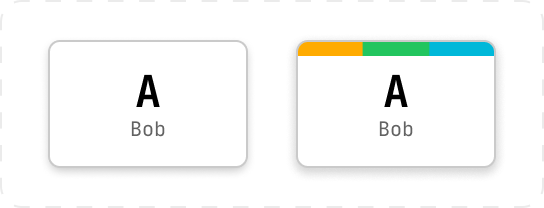
\includegraphics[width=0.5\textwidth]{images/vrcholy1}}
    %popis obrazku
    \caption[Prvý návrh vizuálu vrcholov.]{Prvý návrh vizuálu vrcholov.}
    %id obrazku, pomocou ktoreho sa budeme na obrazok odvolavat
    \label{obr:vrch_navrh_1}
\end{figure}

Použitie týchto vrcholov na grafovú reprezentáciu konkrétneho binárneho predikátu znázorňuje obrázok \ref{obr:basic_navrh_1}. Hrany sú reprezentované šípkami, kde smer šípky upresňuje vzťah medzi prvkami. V pravej časti obrázka sa nachádza zoznam unárnych predikátov spolu s ich príslušnými farbami. Medzi predikátmi, ktoré sa majú zobraziť, je užívateľovi umožnené filtrovať zaškrtnutím k nemu prislúchajúceho políčka.

\begin{figure}
    \centerline{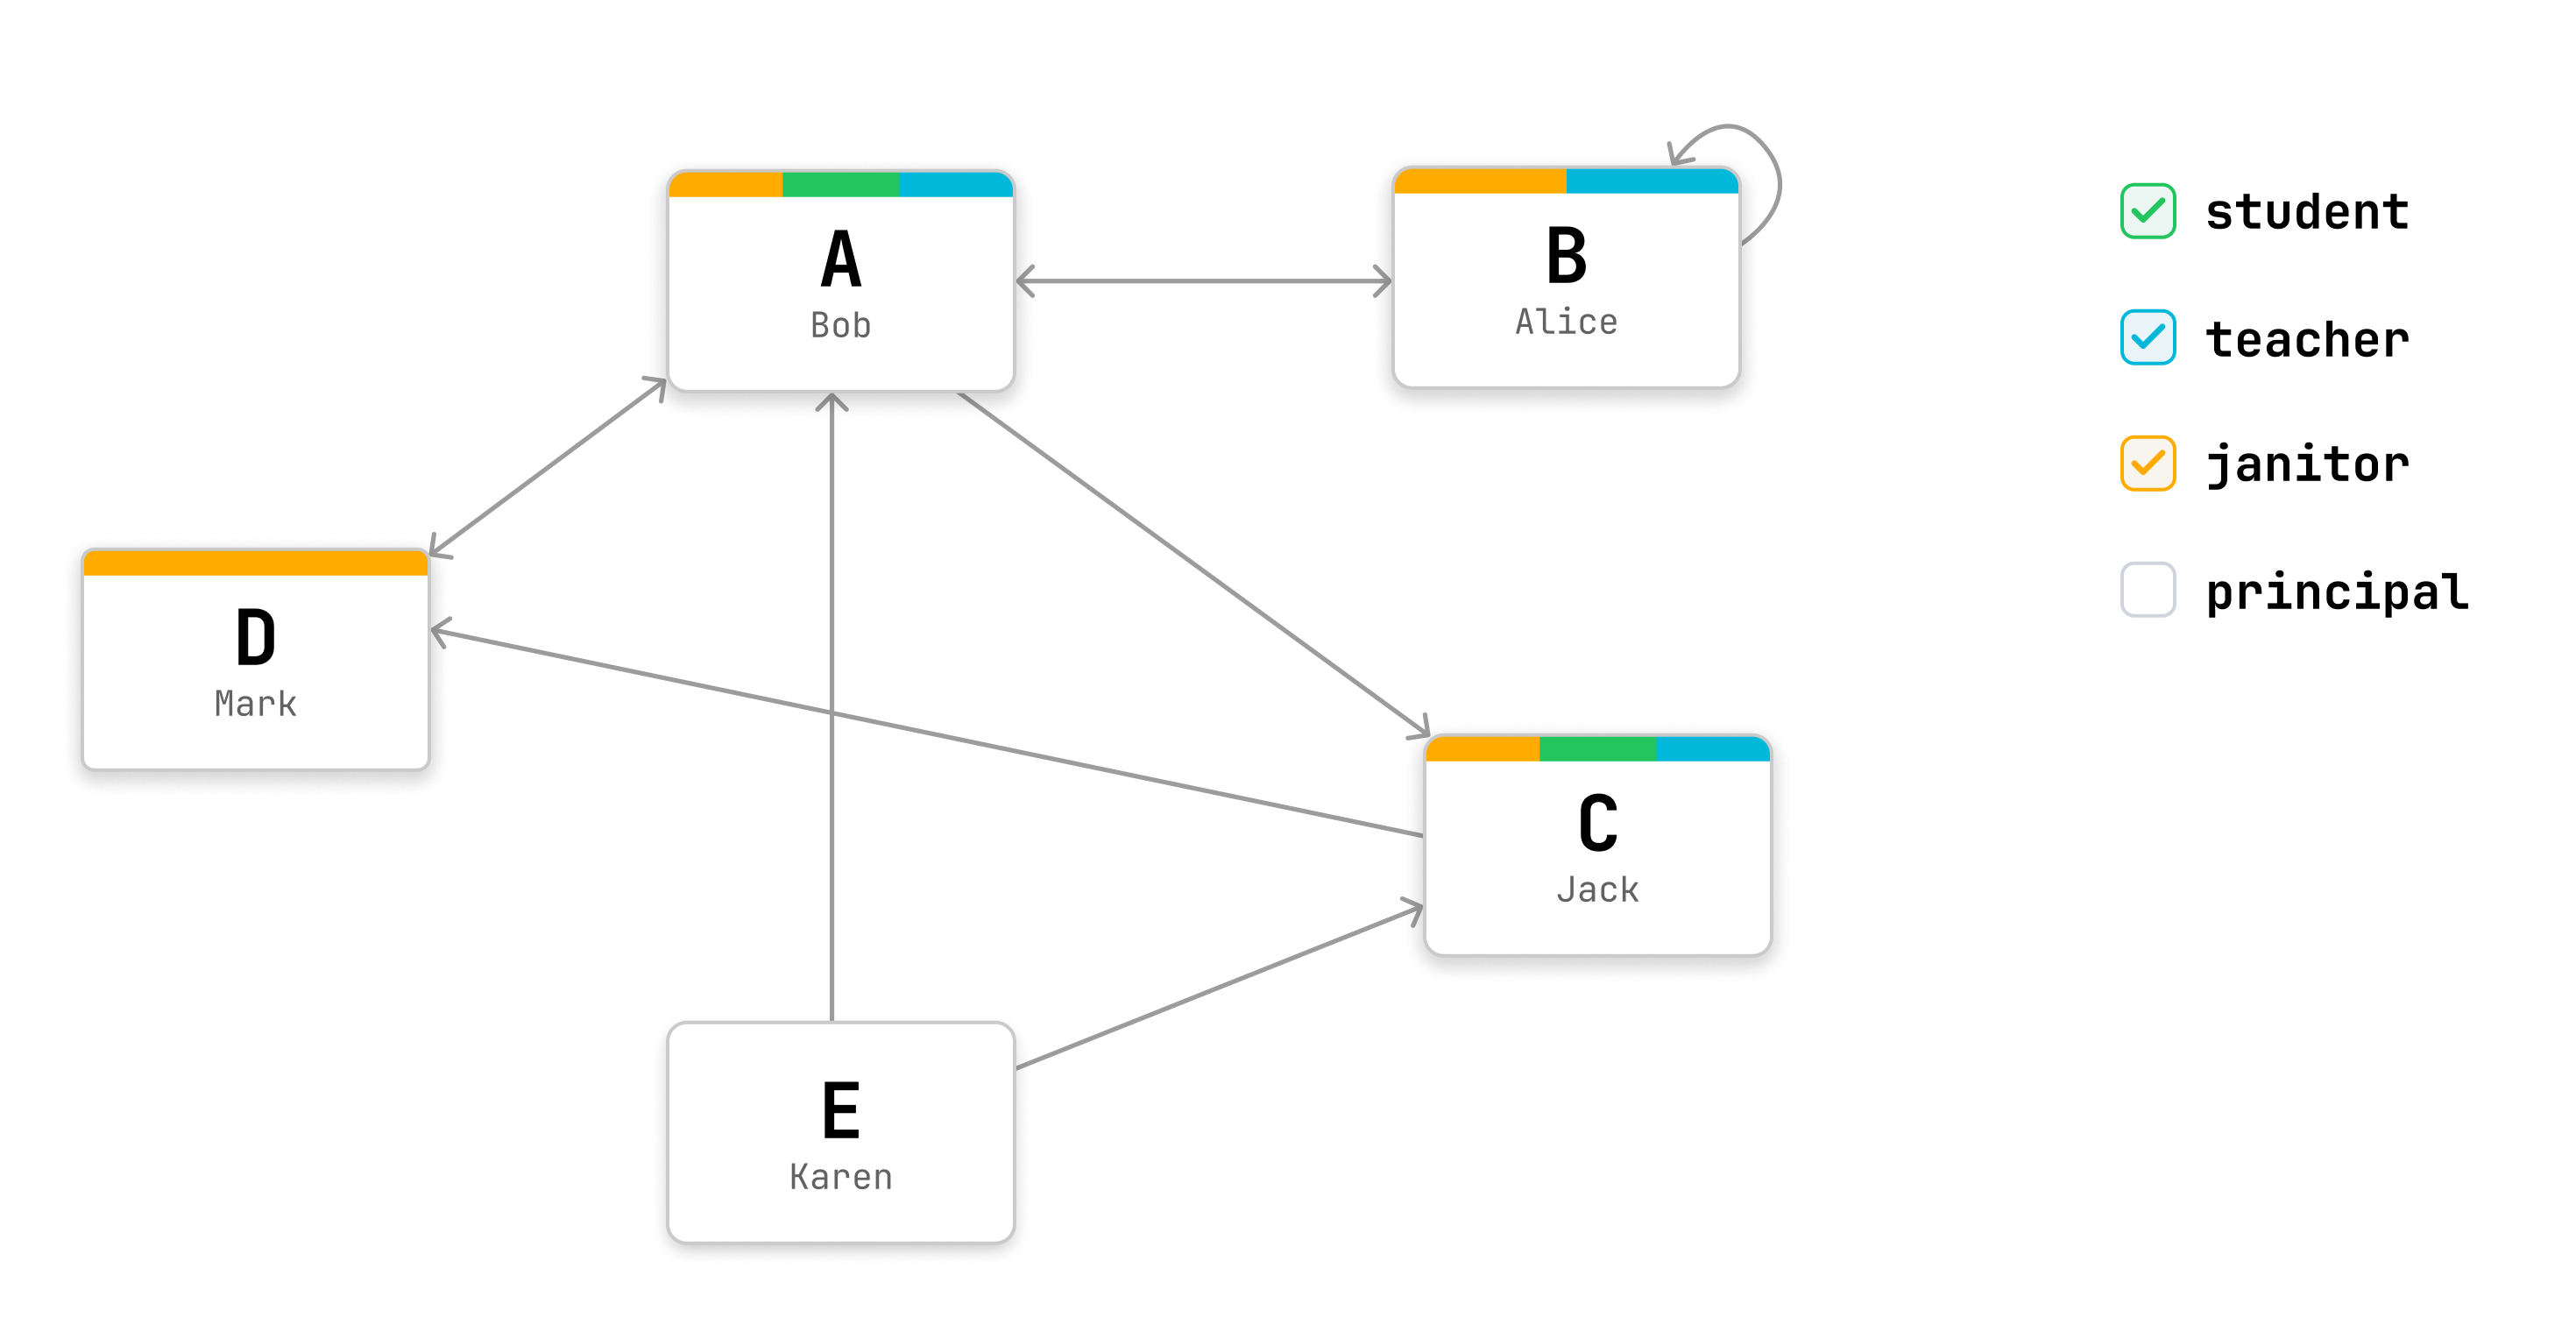
\includegraphics[width=1\textwidth]{images/basic1}}
    %popis obrazku
    \caption[Prvý návrh vizuálu jednoduchého grafu.]{Prvý návrh vizuálu orientovaného grafu.}
    %id obrazku, pomocou ktoreho sa budeme na obrazok odvolavat
    \label{obr:basic_navrh_1}
\end{figure}

\subsection{Bipartitný graf}
\label{bsec:bipartite_graph_navrh}

Zatiaľ čo orientovaný graf je vhodný na získanie všeobecného prehľadu o vzťahoch vyskytujúcich sa v binárnych predikátoch, bipartitný graf má potenciál poskytnúť lepší náhľad na viac špecifické vlastnosti. Napríklad v kontexte zobrazení to môžu byť vlastnosti ako surjektívnosť alebo bijektívnosť. Všeobecne sa však nemusíme obmedzovať len na zobrazenia. Na dosiahnutie zaujímavých výsledkov stačí, aby sa skúmané prvky dali vhodne rozdeliť do dvoch zmysluplných skupín. Úlohou pri tejto grafovej reprezentácii je teda prispôsobiť rozhranie grafu skúmaniu takýchto vlastností.

Základné prvky grafu, ako vrcholy a hrany, sú v zásade zhodné s tými z predošlej reprezentácie. V tomto prípade sa ale vyžaduje, aby boli prvky domény rozdelené do dvoch vizuálne odlíšiteľných celkov (neznamená to však, že musia byť disjunktné). Ďalším rozdielom je spôsob vytvárania hrán. Tie sa dajú vždy vytvárať iba z jednej, predom určenej skupiny, nikdy nie z oboch. Taktiež sa hrany nedajú vytvárať medzi prvkami v rovnakej skupine. Práve tieto obmedzenia robia graf vhodnejší na skúmanie vlastností zobrazení, keďže jeden celok si môžeme predstaviť ako definičný obor (z neho hrany vytvárame) a druhý ako obor hodnôt.

Mnou navrhnuté riešenie možno vidieť na obrázku \ref{obr:bipartite_navrh_1}. Hrany reprezentujú šípky smerujúce zľava doprava. Vrcholy sú rozdelené do dvoch stĺpcov, čo je naznačené aj ich rozdielnou farbou. Každý stĺpec reprezentuje ľubovoľnú podmnožinu prvkov danej domény. Užívateľovi je tiež umožnené meniť poradie vrcholov, ale iba v rámci jeho skupiny, presúvanie medzi nimi nie je dovolené. Vynechaný je panel predstavujúci unárne predikáty, keďže je nateraz otázne, aký veľký by bol jeho prínos pri skúmaní vzťahov špecifických pre bipartitný graf. Posledný, menej výrazný vrchol je iný od ostatných, pretože slúži ako tlačidlo na pridávanie nových prvkov do príslušného stĺpca. Spôsob pridávania vrcholov by mal byť implementovaný ako zoznam, resp. filter, doteraz nepridaných prvok, z ktorých si bude môcť užívateľ vybrať.

\begin{figure}
    \centerline{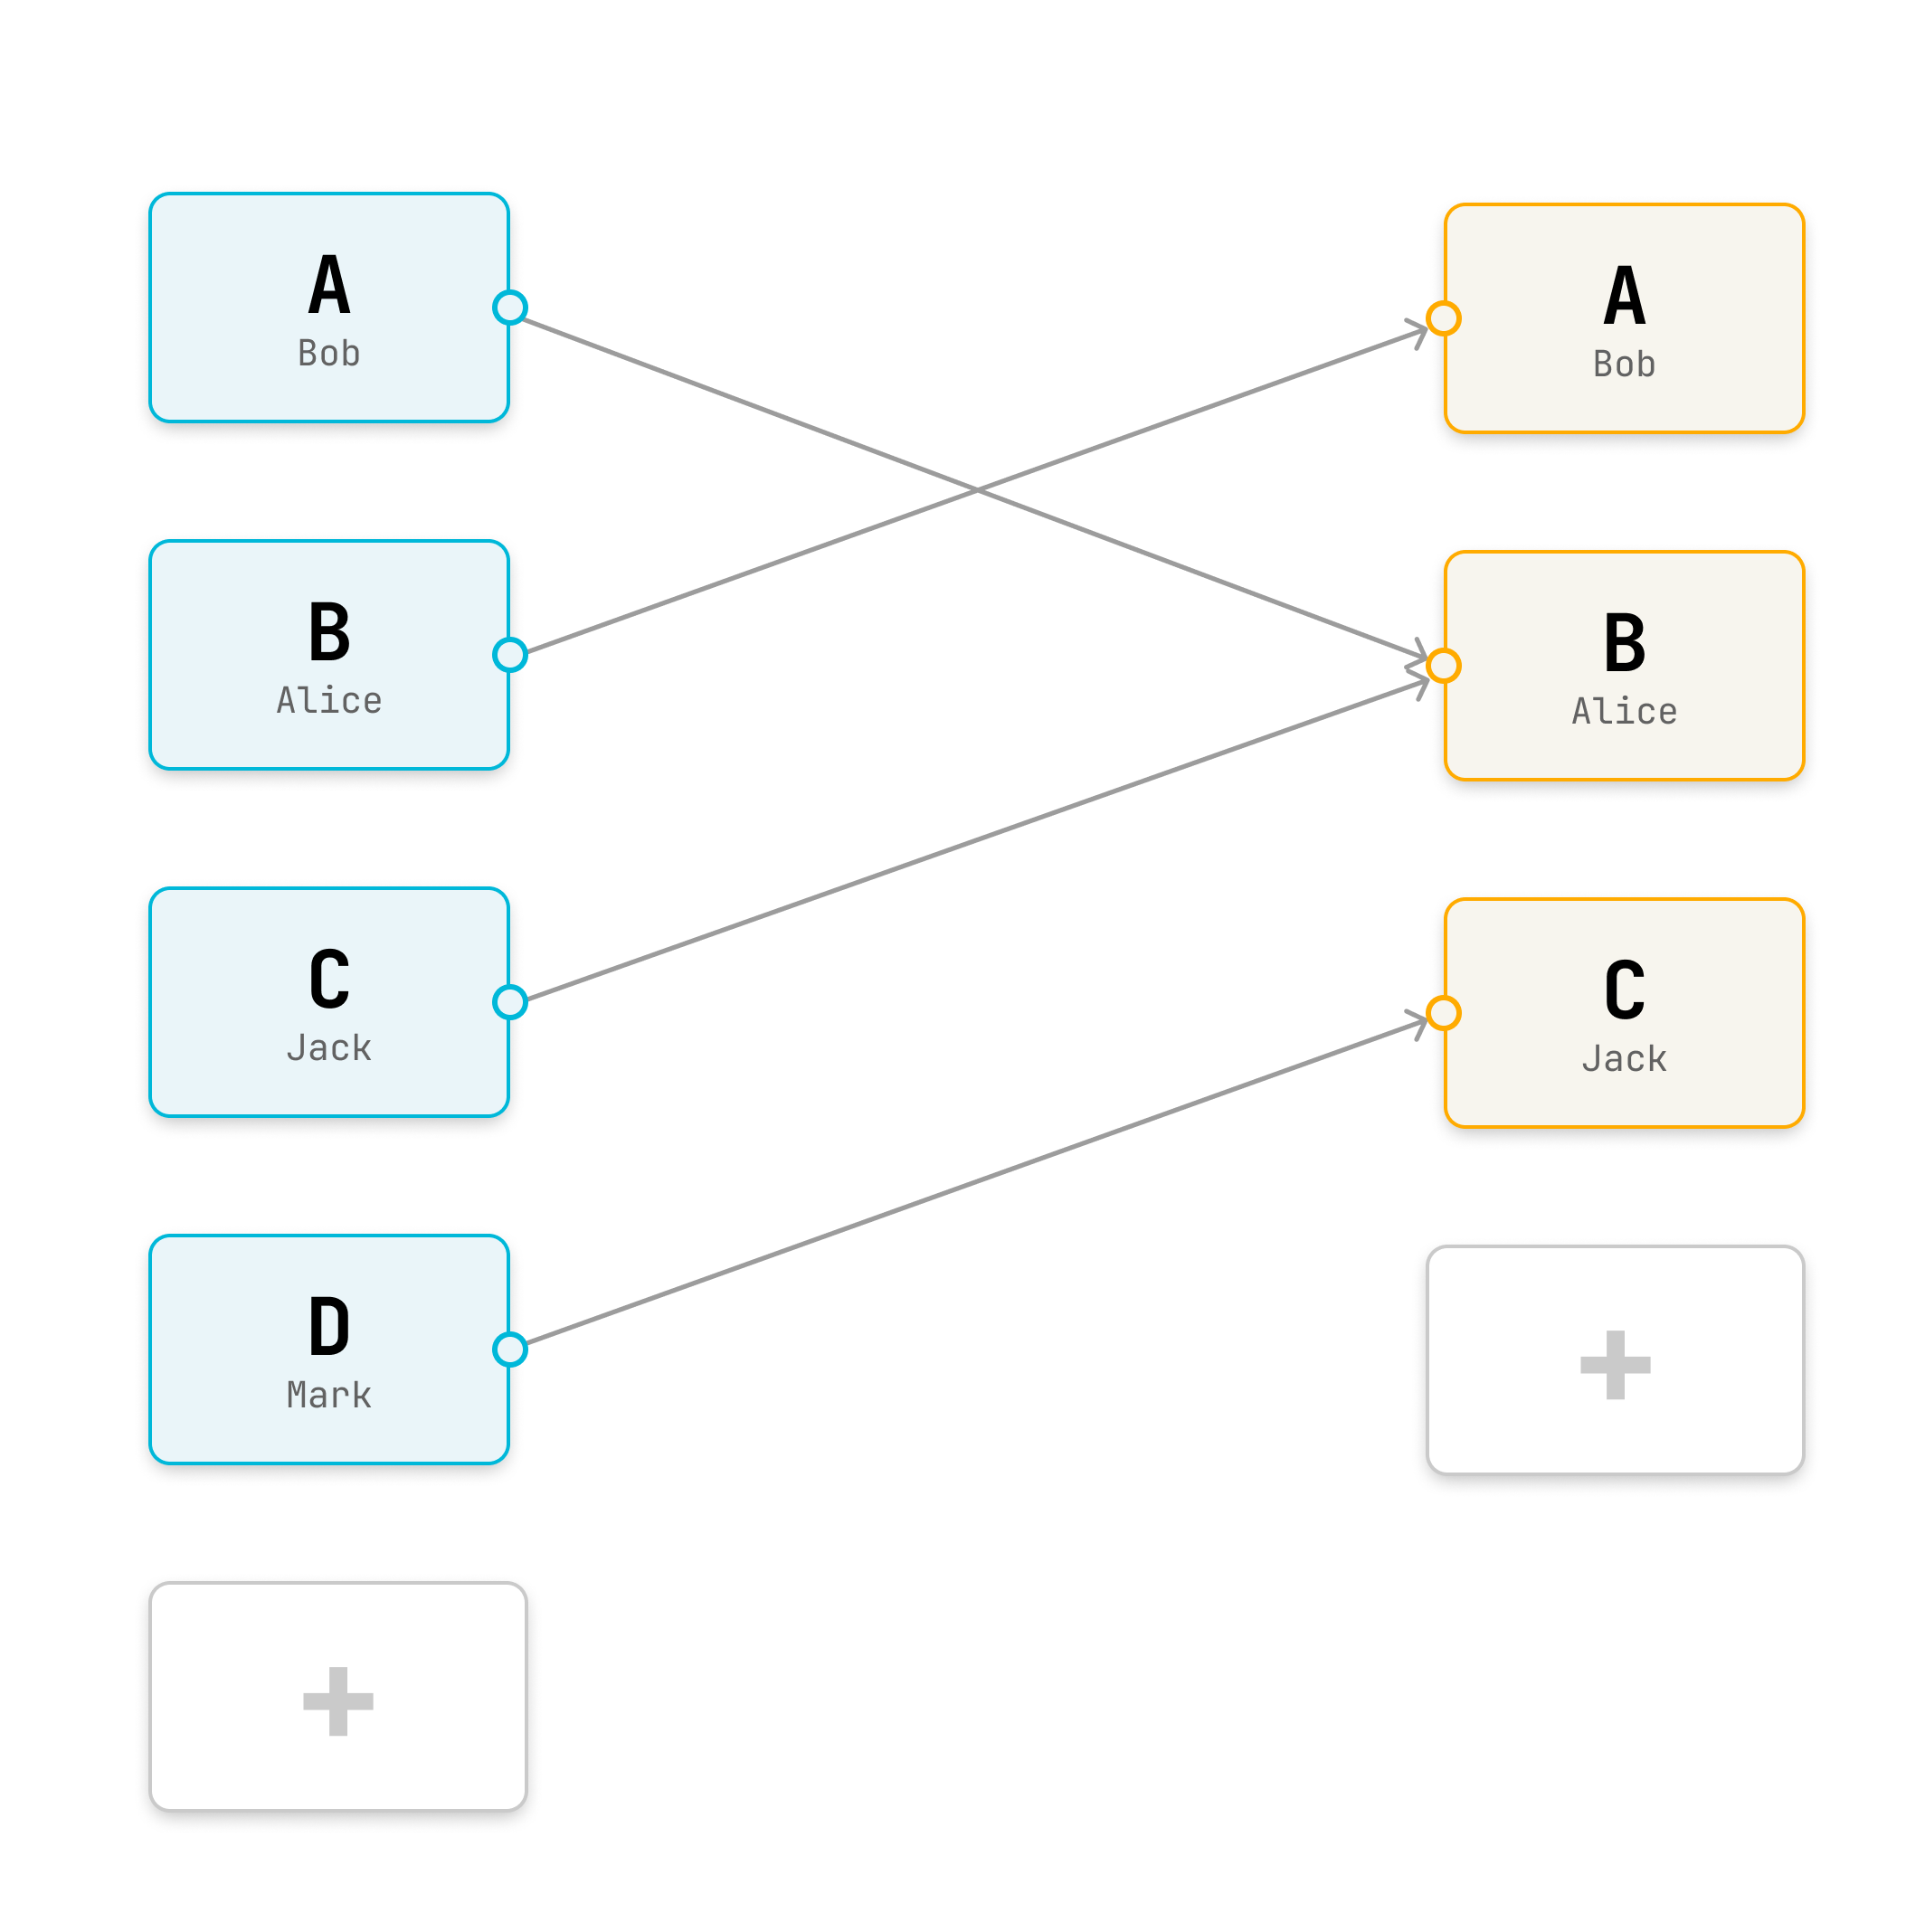
\includegraphics[width=0.7\textwidth]{images/bipartite1.png}}
    %popis obrazku
    \caption[Prvý návrh vizuálu pre bipartitný graf.]{Prvý návrh vizuálu pre bipartitný graf.}
    %id obrazku, pomocou ktoreho sa budeme na obrazok odvolavat
    \label{obr:bipartite_navrh_1}
\end{figure}

\subsection{Hasseho diagram}
\label{sec:hasse_diagram_navrh}

Výhodou Hasseho diagramu je jeho schopnosť výrazne zjednodušiť a sprehľadniť prácu s čiastočnými usporiadaniami. Samotný orientovaný graf nie je ideálny pre tento účel z viacerých dôvodov. Napríklad pri čiastočných usporiadaniach s väčším počtom prvkov sa stáva neprehľadným, keďže vždy zobrazuje všetky hrany, čo často nie je nutné. Ďalším je, že aj jednoduchá úprava takéhoto čiastočného usporiadania môže v orientovanom grafe znamenať potrebu ručne vytvoriť množstvo nových hrán, kvôli nutnosti zachovania tranzitivity, čím sa uberá na použiteľnosti. Cieľom je navrhnúť vhodnú grafovú reprezentáciu Hasseho diagramu, ktorá (ako už bolo spomínané v podkapitole \ref{sec:reprezentacie}) dokáže s týmito problémami pomôcť.

Vrcholy a hrany grafu ostanú opäť výrazne nezmenené, no kvôli prehľadnosti bude zásadné dodržať správnu vertikálnu hierarchiu vrcholov, ktorá je tiež súčasťou konštrukcie Hasseho diagramu. Zámerom však nie je užívateľa akokoľvek obmedzovať za účelom dodržiavania tejto hierarchie, ako tomu bolo v bipartitnom grafe, ale poskytnúť mu dobrý základ rozmiestnenia vrcholov, ktorý je ďalej prispôsobiteľný vlastným predstavám. Dôležitá bude tiež korektná implementácia zvyšných vlastností Hasseho diagramu, ako aj validácia nových hrán pridaných užívateľom. Dôraz na validáciu je kladený hlavne kvôli tomu, že pridaním nesprávnej hrany môže reprezentácia prestať dávať zmysel.

\begin{figure}
    \centerline{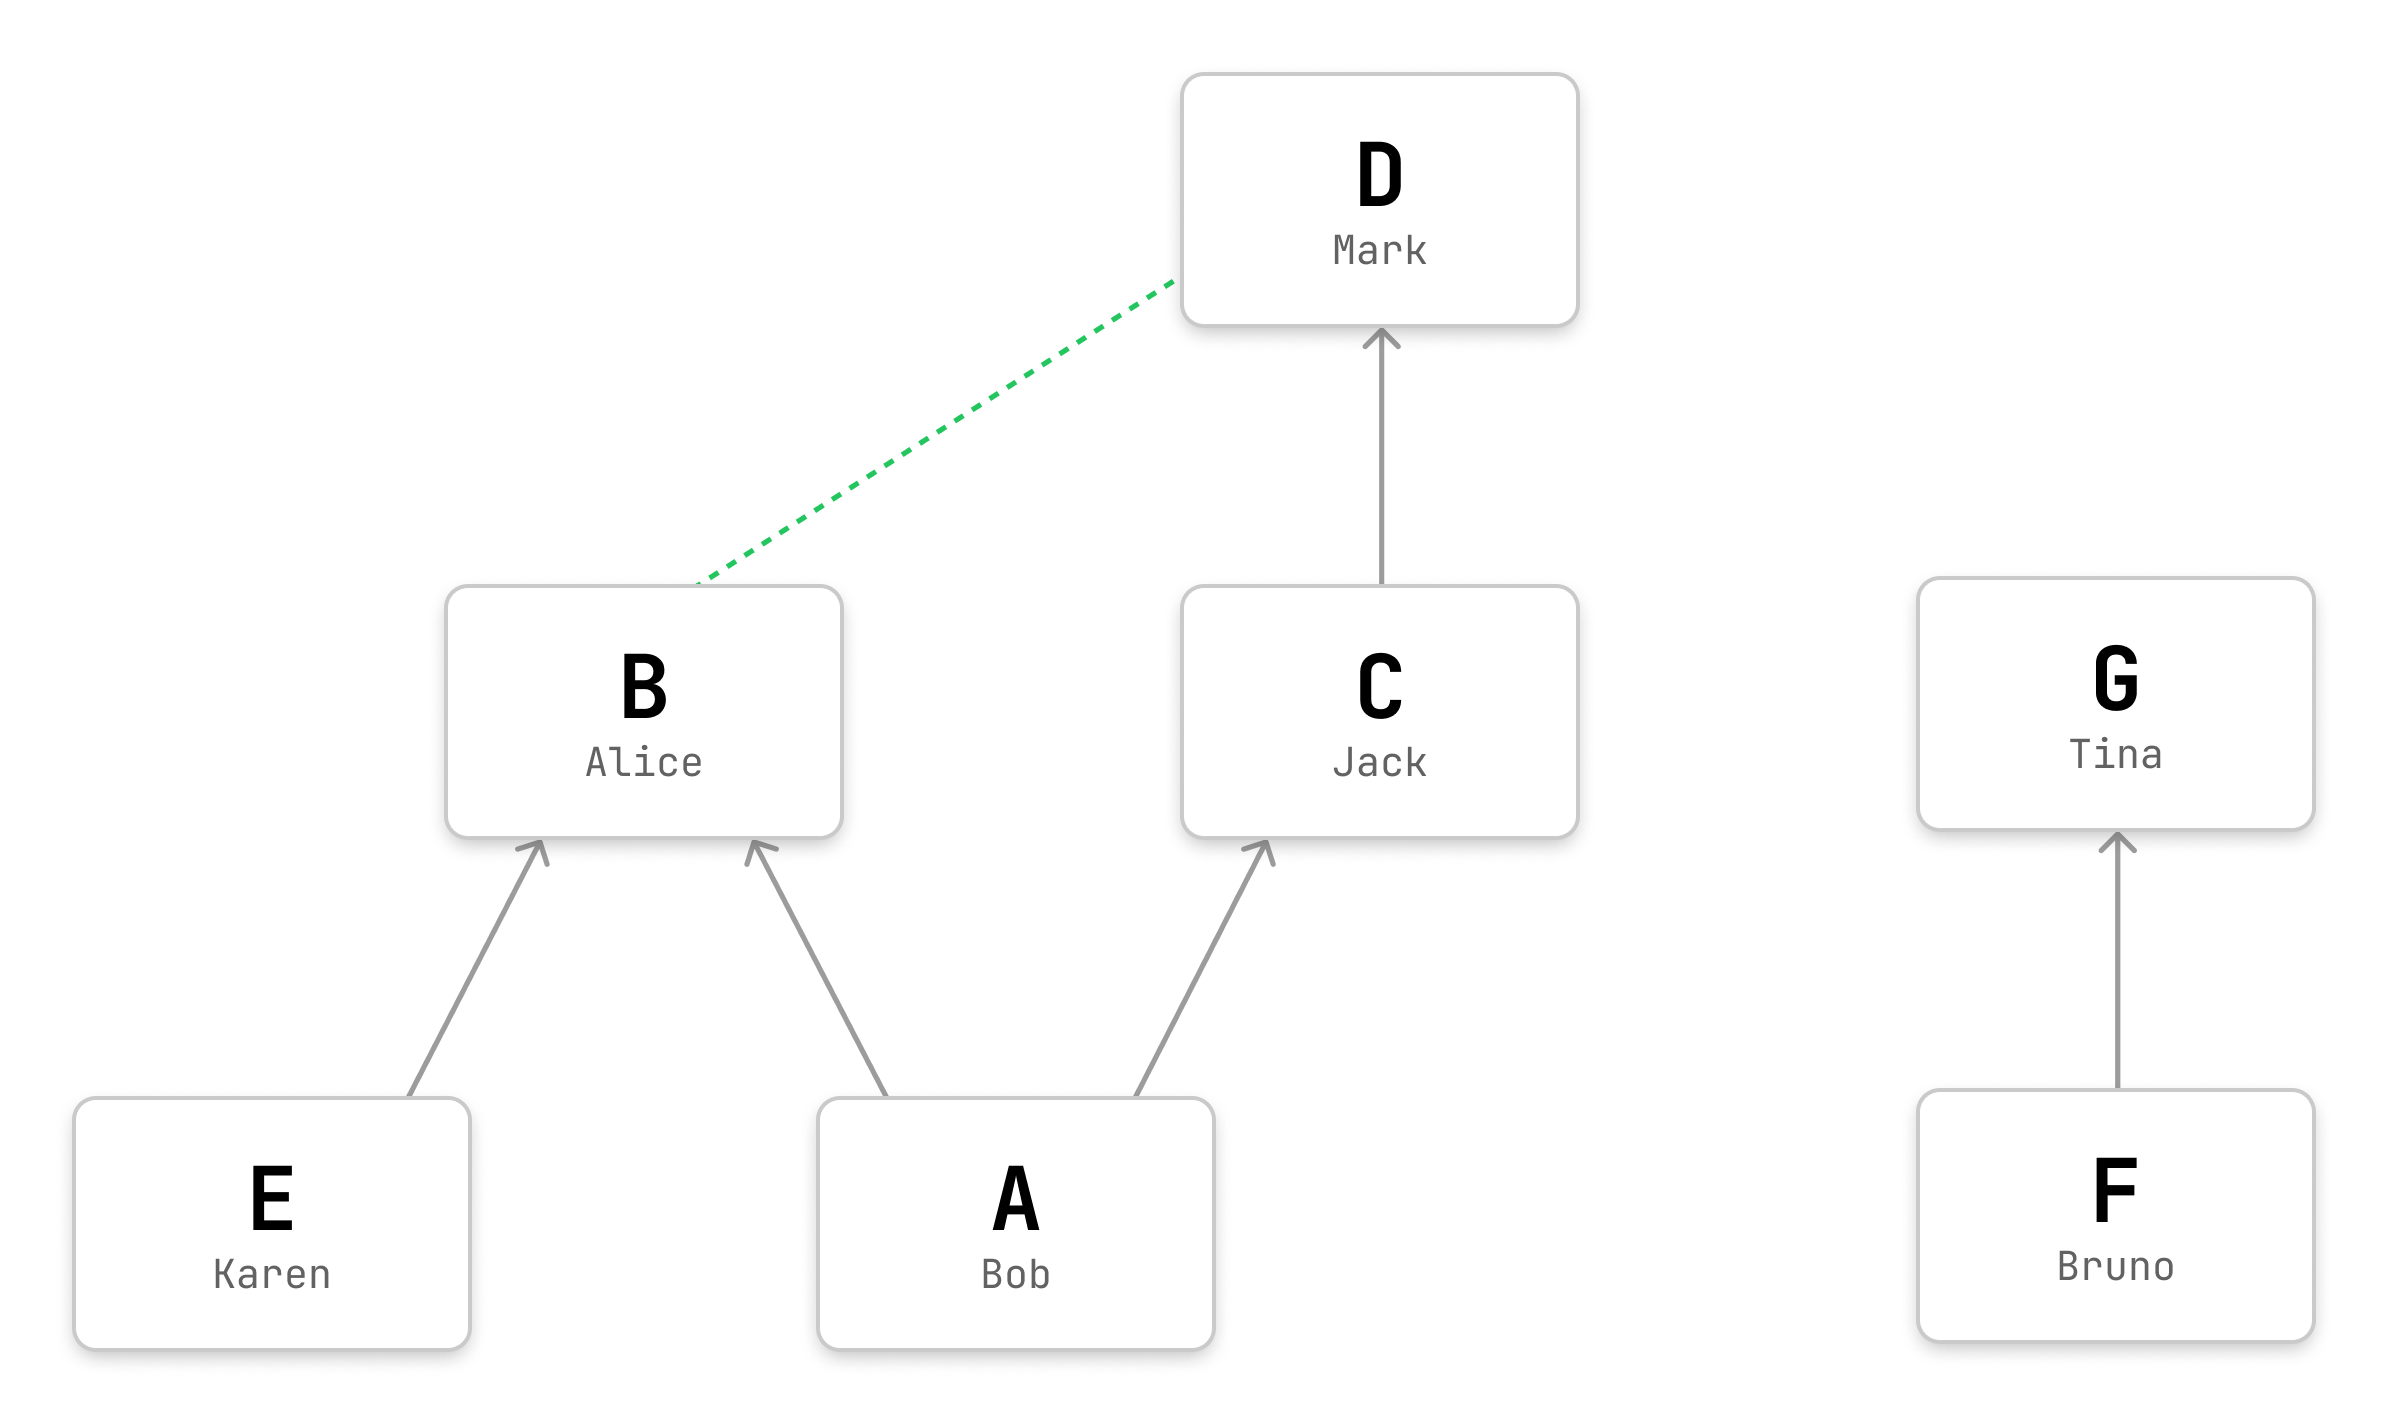
\includegraphics[width=0.75\textwidth]{images/hasse1.png}}
    %popis obrazku
    \caption[Prvý návrh vizuálu pre Hasseho diagram.]{Prvý návrh vizuálu pre Hasseho diagram.}
    %id obrazku, pomocou ktoreho sa budeme na obrazok odvolavat
    \label{obr:hasse_navrh_1}
\end{figure}

Môj návrh možno vidieť na obrázku \ref{obr:hasse_navrh_1}. Viditeľná je jasná hierarchia vrcholov s orientovanými hranami smerujúcimi nahor. Zelenou prerušovanou čiarou je užívateľovi naznačená korektnosť hrany, ktorú sa práve snaží pridať (tu je hrana v poriadku). V opačnom prípade by hrana bola červená a pokus o jej vytvorenie by nemal žiadny účinok. Ostatné prvky sú podobné ako v predošlých reprezentáciách.

\section{Tabuľkové editory}
\label{sec:plan-table-editors}
TODO
\subsection{Maticový editor}
TODO
\subsection{Databázový editor}
TODO

\section{Editor interpretácií funkcií}
TODO

\section{Spoločné rozhranie editorov}
\label{sec:plan-editors-ui}
TODO

\section{Nový stav aplikácie}
TODO

\section{Queries}
\label{sec:plan-queries}